\section{Q3: Do Operators Fight Back?}
\label{sec:q3}

In the active cohort, 26 satellites showed manoeuvres: the 25 Starlinks and one 1967
calibration satellite whose ``manoeuvres'' turned out to sit on steady free-drag decay, which the
free-drag screen removes. Question~3 is therefore an exploratory Starlink study. After the
screens, 21 Starlinks contribute across the 20 storms. Coverage is uneven, because not every
satellite covers every storm's windows.

Table~\ref{tab:q3} and Fig.~\ref{fig:offset} give the result. With the passive model-error
correction, the offset ratio is 1.17 (95\% CI 0.97--1.36). At the point estimate, Starlinks lose
no more altitude around storms than in their normal pre-storm routine, and the interval still
allows an offset slightly short of complete. Almost all of it happens during the storm (ducking
part 1.16, CI 1.05--1.27), while the recovery part is about zero ($+0.01$, CI $-0.22$ to
$+0.21$). At TLE resolution, then, the satellites make up the loss while the storm is still
going, not by climbing back afterwards.

The result holds without May and October 2024 (1.25, CI 1.08--1.41) and without the six storms
whose pre-storm quiet ap was raised by an earlier storm (1.15, CI 1.04--1.26). In that second
subset the recovery part is $+0.15$ (CI 0.04--0.28), so a small part of the offset may happen
after the storm. Values above 1 are larger than the scatter on storm-free dates and could mean
slightly over-compensating thrust or the smoothing in mean-element TLEs. Since the lower end of
the main interval is just below 1, our reading is careful: for the selected satellites and
operating periods, the observed orbit changes are consistent with an approximately complete
offset of the model-predicted storm loss. An offset ratio is not a measurement of thrust. TLEs
alone cannot separate thrust, attitude changes, routine manoeuvre timing and model error.

\begin{table}[t]
\caption{Starlink operator offset ratio (21 satellites)}
\label{tab:q3}
\centering
\small
\begin{tabular}{@{}lcc@{}}
\toprule
Run & Offset & 95\% CI \\
\midrule
All 20 storms, uncorrected & 1.19 & 0.77--1.64 \\
All 20 storms, corrected & \textbf{1.17} & 0.97--1.36 \\
\quad ducking part & 1.16 & 1.05--1.27 \\
\quad recovery part & $+0.01$ & $-0.22$ to 0.21 \\
Without May/Oct 2024 & 1.25 & 1.08--1.41 \\
Undisturbed quiet ap (14 storms) & 1.15 & 1.04--1.26 \\
\bottomrule
\end{tabular}
\end{table}

\begin{figure}[t]
\centering
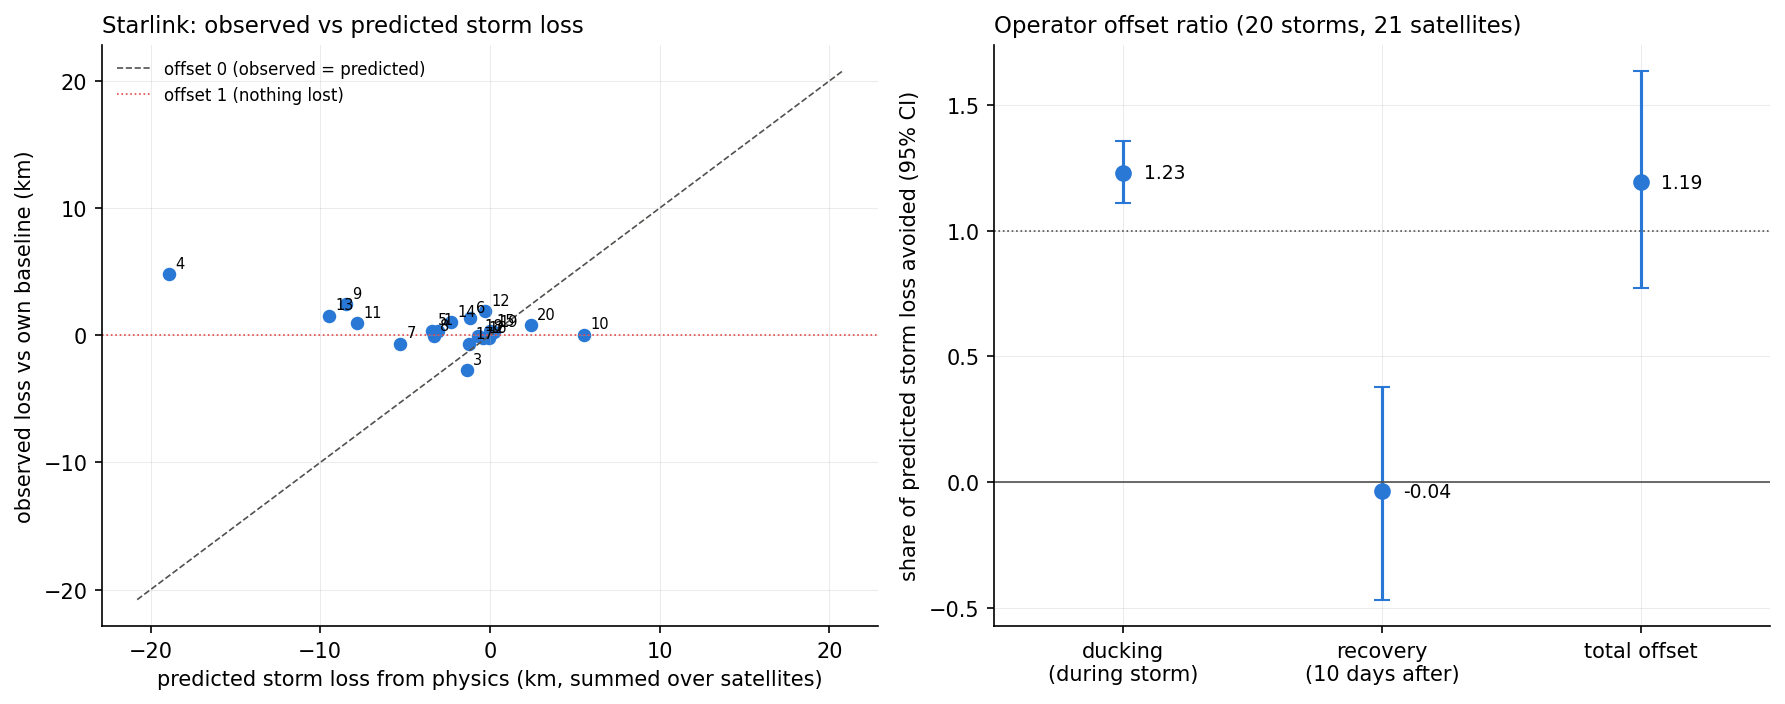
\includegraphics[width=\columnwidth]{fig7_operator_offset.png}
\caption{Starlink offset (uncorrected run: total 1.19, ducking 1.23, recovery $-0.04$; the
corrected values are in Table~\ref{tab:q3}). Left: observed against predicted storm loss per
storm, summed over satellites; points near the dotted line lost nothing. Right: ducking, recovery
and total offset with 95\% storm-clustered intervals.}
\label{fig:offset}
\end{figure}

Five caveats apply. First, this is one operator. Second, drag sensitivity comes from the
catalogue scaled by passive-object fits. In a pre-freeze run, scaling it by $\pm25\%$ moved the
ratio to 1.15--1.25, but a badly wrong scale could fake an offset. Third, the screens that drop
deorbits and orbit raises are based on observed altitude, so they could also drop periods of poor
compensation. Fourth, the passive model-error correction is carried over in m/day by storm class
and altitude band, not scaled to each satellite's drag sensitivity. Fifth, the intervals hold the
predicted loss fixed, and a placebo on Starlinks in free drag is compatible with zero but too
imprecise to really validate the method.
